\definecolor{qqqqcc}{rgb}{0,0,0.8}
%dash pattern=on 5pt off 2pt
%[fill = white, rounded corners = 5pt, inner sep=0.8pt]
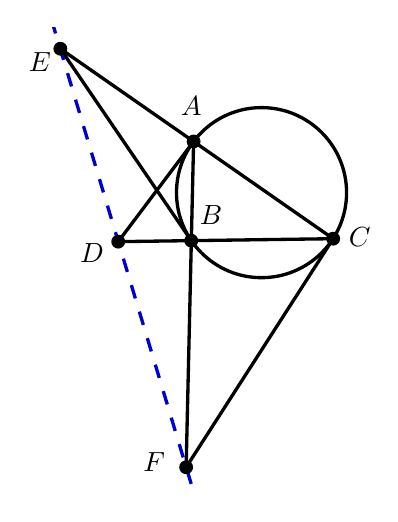
\begin{tikzpicture}[scale = 0.25]
    \clip(-10.02,-12.9) rectangle (7.34,10.77);
    \draw [line width=1.2pt] (1.86,2.39) circle (4.32cm);
    \draw [line width=1.2pt] (-8.36,9.7)-- (5.5,0.05);
    \draw [line width=1.2pt] (-8.36,9.7)-- (-1.71,-0.05);
    \draw [line width=1.2pt] (-5.42,-0.1)-- (5.5,0.05);
    \draw [line width=1.2pt] (-5.42,-0.1)-- (-1.59,4.99);
    \draw [line width=1.2pt] (-1.97,-11.56)-- (5.5,0.05);
    \draw [line width=1.2pt] (-1.97,-11.56)-- (-1.59,4.99);
    \draw [line width=1.2pt,dash pattern=on 5pt off 5pt,color=qqqqcc,domain=-10.02:7.34] plot(\x,{(-115.81-21.26*\x)/6.4});
    \begin{scriptsize}
        \normalsize
        \fill [color=black] (-1.59,4.99) circle (10.0pt);
        \draw[color=black] (-1.71,6.81) node {$A$};
        \fill [color=black] (-1.71,-0.05) circle (10pt);
        \draw[color=black] (-0.7,1.24) node {$B$};
        \fill [color=black] (5.5,0.05) circle (10pt);
        \draw[color=black] (6.85,0.11) node {$C$};
        \fill [color=black] (-8.36,9.7) circle (10pt);
        \draw[color=black] (-9.4,9) node {$E$};
        \fill [color=black] (-5.42,-0.1) circle (10pt);
        \draw[color=black] (-6.75,-0.69) node {$D$};
        \fill [color=black] (-1.97,-11.56) circle (10pt);
        \draw[color=black] (-3.59,-11.3) node {$F$};
    \end{scriptsize}
\end{tikzpicture}